\newpage
\section{Durchführung}
Folgendes soll untersucht werden:
\begin{enumerate}
    \item Messung: Einfluss der Windungszahl $n$ auf die Federkraft $F$. Dies soll dem zusätzlichen
    Materialverbrauch gegenübergestellt werden.
    \item Messung: Einfluss der Federdicke $D$ auf die Federkraft $F$. Dies soll dem zusätzlichen
    Materialverbrauch gegenübergestellt werden.
    \item Fazit: Kompinierung der Parameter Windungszahl $n$ und Federdicke $D$ für ein minimum
    an Materialverbrauch bei vorgegebener Federkrafttoleranzbereich.
\end{enumerate}
Als Basis verwende man eine zu der Zeichnung und den Größen passende Zugfeder. Diese
wird zunächst gewogen (mehrere Federn und dann mitteln) und ihre Federkraft $F_{Basis}$
geprüft.\\
Nun werden jeweils 5 Federn mit varriierender Windungszahl $\Delta n$ produziert und deren
Gewicht sowie Federkraft $F_{\Delta n}$ vermessen.
Danach wird die Maschine auf die Basislage zurückgestellt. NUn wird der Paramter 
der Federdicke um $\Delta d$ varrieriert und resultierende Federkraft $F_{\Delta d}$
vermessen.  

\newpage

\subsection{Die Feder}

Betrachtet wird eine Trompetenfeder, welche in der Möbelbeschlagindustrie in Schubladeneinzugsystemen
verwendet wird. 
Der Federtyp zeichnet sich durch die nicht klassische Ösenform aus, welche die Problematik des Ösenbruchs löst.\\

Wichtig ist anzumerken, dass die Ruhelänge $L_0$ in der Praxis legiglich als anzustreben gilt.
Die Länge der Zugfeder vergrößert bei Belastung, deshalb bedarf es keiner festgeschrieben Maximallänge für $L_0$, da
der Einbauraum stehts auf eine großerwerdene Feder ausgelegt ist.  
\newline

\begin{center}
    \makebox[\textwidth]{
        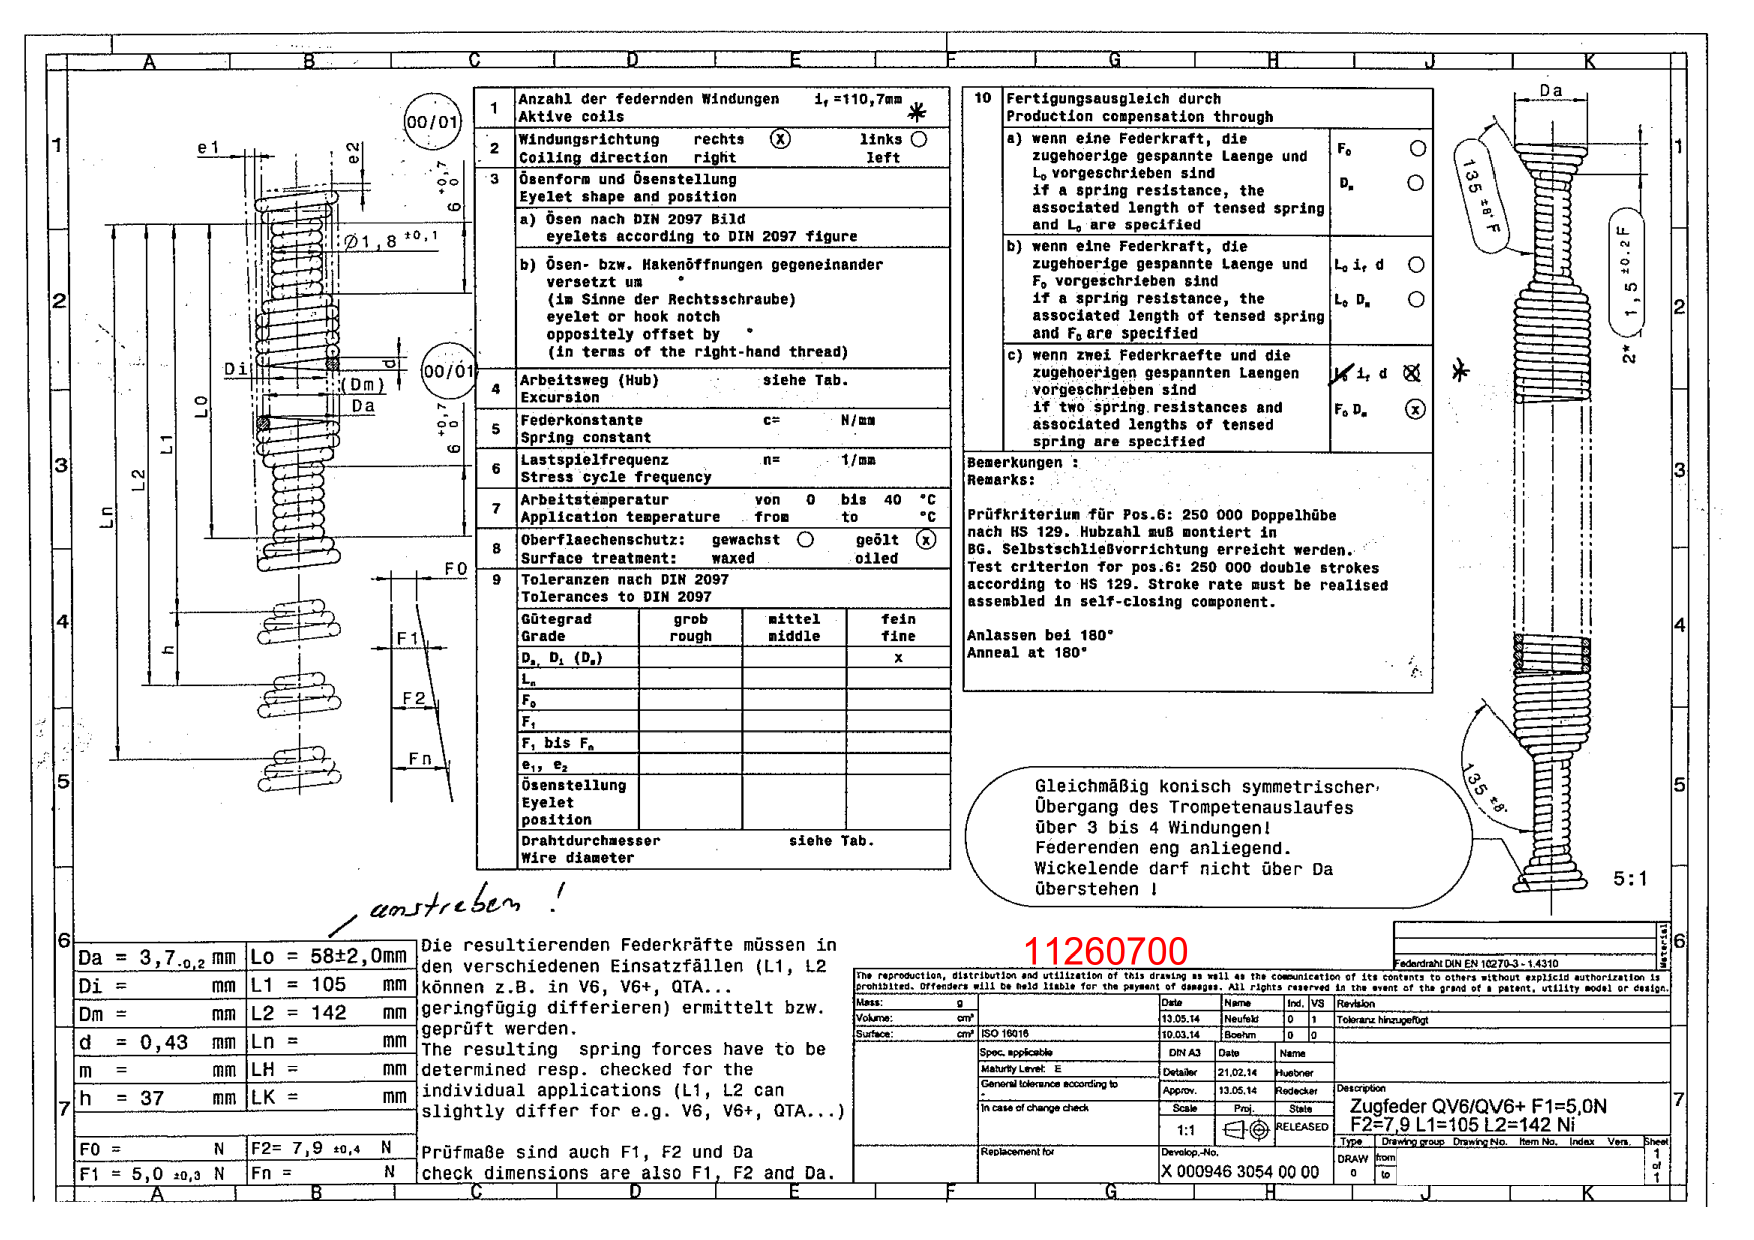
\includegraphics[width=\paperwidth]{bilder/zeichnung_11260700.pdf}
        }
\end{center}
\newpage
Die Zeichnung zeigt die Feder mit einem Ausdurchmesser $D_a$ von $3,7\;\text{mm}$.\\ 
Als Basisfeder wird hier der Ausdurchmesser von $3,5\;\text{mm}$ verwendet.\\


Im folgenden kann die Feder als zylindrische Feder betrachtet werden,
da die Belastung in der Größenordung liegt, sodass der zu federnde Anteil nicht 
vom Trompentenanteil (gemeint sind hier die Ösenteile am Ende der Feder)
ausgeführt wird.

\label{sec:Durchfuehrung}